\section{Time-of-Flight Magnetic Resonance Angiography}
\label{chapter3}
% Aim for 5-7 pages

As discussed briefly previously, Time-of-Flight (TOF) Magnetic Resonance Angiography (MRA) is an imaging modality used for diagnosis of UIAs. The following chapters will lay out the specifics on the deep learning methods used to segment UIAs on these images, however it is also valuable to go deeper into the acquisition of these images, as well as discuss and analyze the specific images used.

3D TOF-MRA is based on a 3D T1 weighted echo gradient compensated for flow to emphasize the vascular signal relative to the stationary proton signal in surrounding tissues \cite{Rodriguez-Regent2014}. With TOF-MRA it is also simple to provide an assessment of MRA quality based on spatial definition of the various visualized arteries. An example TOF-MRA volume can be seen in Figure \ref{fig:tof-mra-3d-noenhance.png}, however due to the difficulty in visualizing the vessels an enhanced representation is also shown in Figure \ref{fig:tof-mra-3d.png} with increased opacity of the vessels and decreased opacity of the background. A representation of the volume in 3 views (axial, coronal, and sagittal) can also be seen in Figure \ref{fig:tof-3views.png}.

\begin{figure}[htp]
	\centering
	\begin{subfigure}{0.45\linewidth}
		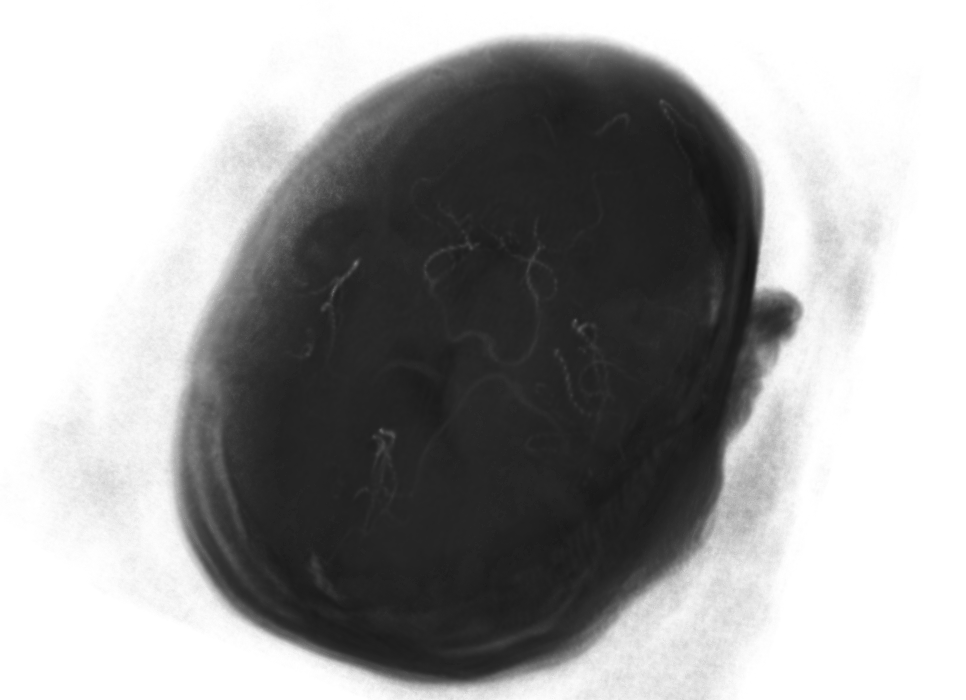
\includegraphics[width=\linewidth]{figures/tof-mra-3d-noenhance.png}
		\caption{}
		\label{fig:tof-mra-3d-noenhance.png}
	\end{subfigure}
	\begin{subfigure}{0.45\linewidth}
		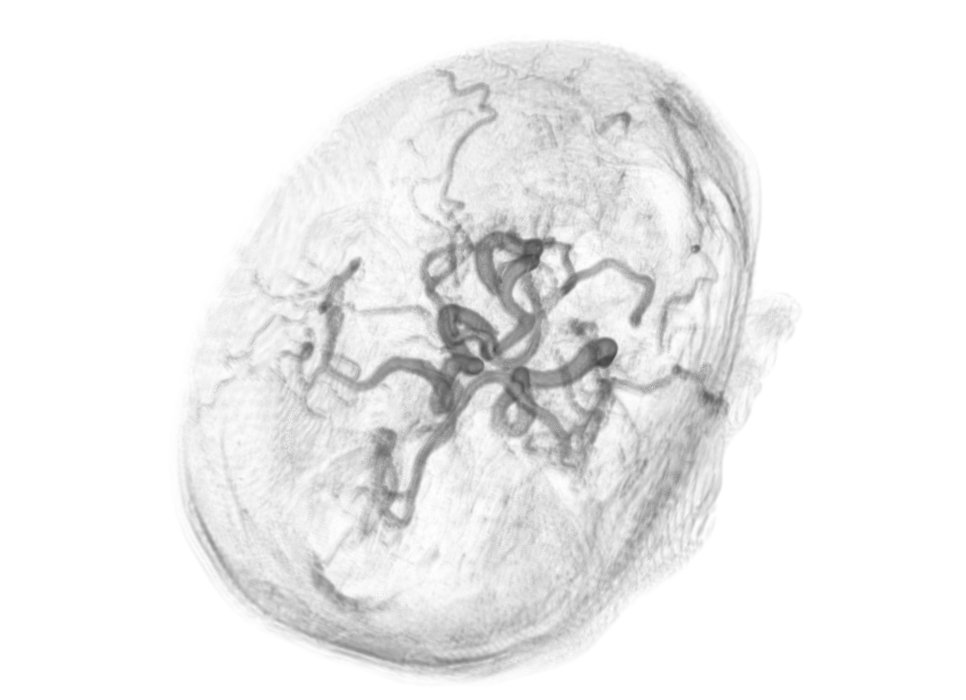
\includegraphics[width=\linewidth]{figures/tof-mra-3d.png}
		\caption{}
		\label{fig:tof-mra-3d.png}
	\end{subfigure}
	\caption[3D TOF-MRA volume]{Two equivalent TOF-MRA volumes, obtained through the MICCAI2020 ADAM challenge run by \citeauthor{Timmins2020} with (a) being a regular volume, and (b) being a volume with enhanced opacity of the cerebrovascular structure.}
\end{figure}

\begin{figure}[htp]
	\centering
	\begin{subfigure}{.33\linewidth}
		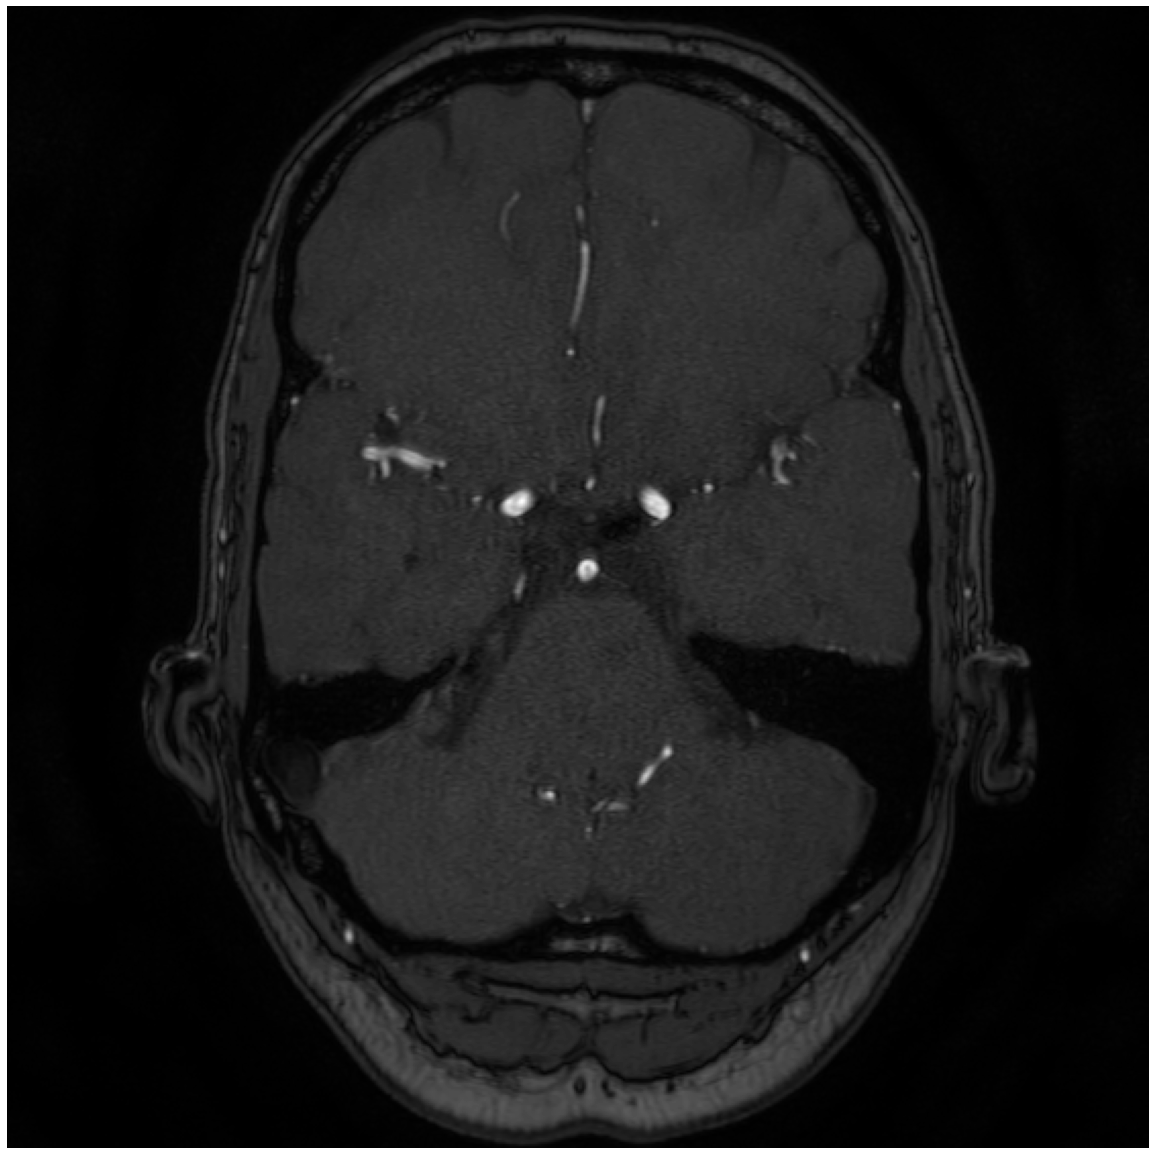
\includegraphics[width=\linewidth]{figures/tof-mra-axial.png}
	\end{subfigure}
	\begin{subfigure}{.63\linewidth}
		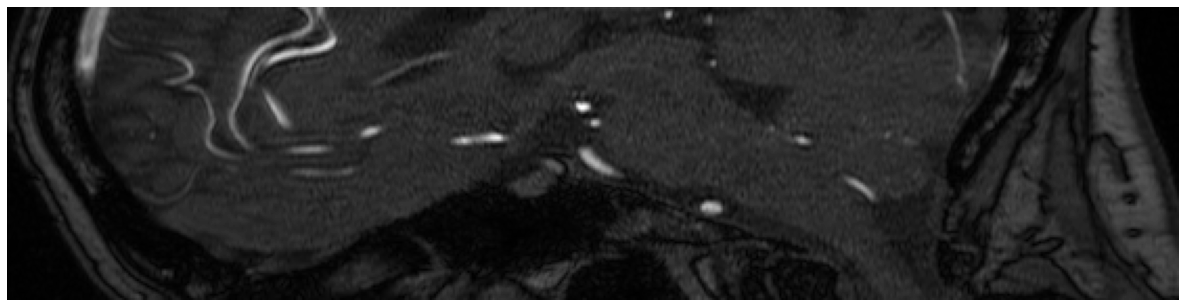
\includegraphics[width=\linewidth]{figures/tof-mra-sag.png}
		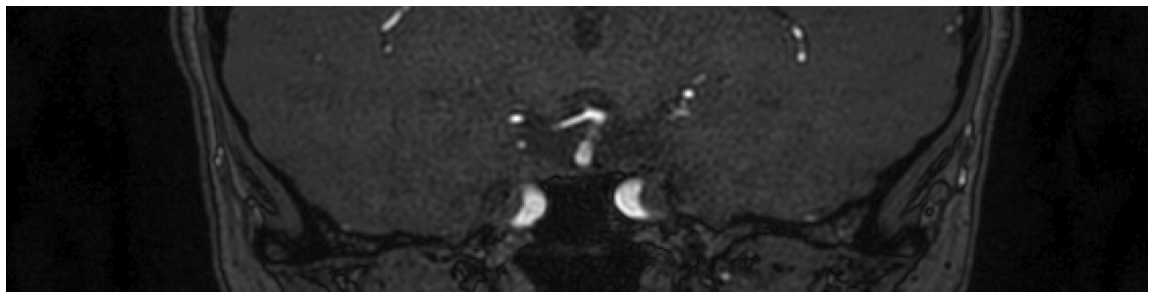
\includegraphics[width=\linewidth]{figures/tof-mra-cor.png}
	\end{subfigure}
	\caption[Axial, sagittal and coronal slices of 3D TOF-MRA]{Three anatomical views of a 3D TOF-MRA volume. Left: axial slice, top right: sagittal slice, bottom right: coronal slice.}
	\label{fig:tof-3views.png}
\end{figure}

\subsection{Aneurysms}
Saccular aneurysms are pathological dilations at major branching brain arteries -- they bulge out at a cerebral artery bifurcation. They contain a distinct neck, connecting the aneurysm to the parent vessel(s), and a larger rounded area called the dome. Non-saccular aneurysms on the other hand are fusiform -- spindle-like -- in shape and involve the parent vessel wall circumferentially. Non-saccular aneurysms are much less common than saccular aneurysms and they also seldom rupture in comparison. The two types of UIAs are shown in Figure \ref{fig:aneurysms.png}.

\begin{figure}[h]
	\centering
	\begin{subfigure}{.45\linewidth}
		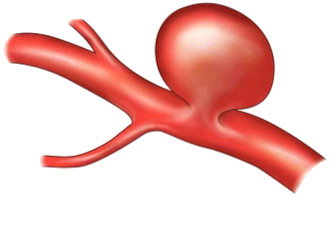
\includegraphics[width=\linewidth]{figures/saccular.png}
		\caption[Saccular aneurysm]{Saccular aneurysm}
	\end{subfigure}
	\begin{subfigure}{.45\linewidth}
		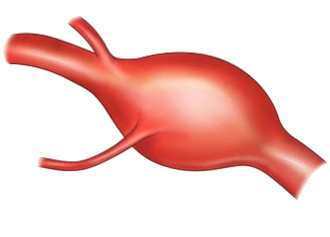
\includegraphics[width=\linewidth]{figures/fusiform.png}
		\caption[Non-saccular aneurysm]{Non-saccular aneurysm}
	\end{subfigure}
	\caption[Types of aneurysms.]{Types of common cerebral aneurysms occurring in cerebral vasculature. Picture adapted from \citeauthor{Withers2013}.}
	\label{fig:aneurysms.png}
\end{figure}

Intracranial aneurysms chiefly develop in the arterial part of the circle of Willis ($70$ to $90\%$ depending on the studies) \cite{Rodriguez-Regent2014}. The circle of Willis being an important junction of arteries at the base of the brain, where the internal carotid arteries branch into smaller arteries supplying oxygenated blood to over $80\%$ of the cerebrum. The specific location of the aneurysm could be further subdivided into various arteries. In $15$ to $20\%$ of cases it is also possible for multiple aneurysms to be present.

Size of UIAs are variant and can also be significantly dependent on the site the aneurysm presents itself. A study conducted on a database of patients between 1967 and 1987 that were treated for aneurysms found the mean size of UIAs to be $7.8$ mm, with a median size of $5$ mm \cite{Weir2002}. Of the same patients, the bulk of aneurysms were $\leq 10$ mm; $27\%$ were $\leq 3$ mm, and $58\%$ were $4$--$10$ mm in size.

The sensitivity and specificity of 3D TOF-MRA to detect the presence of an intracranial aneurysm over 3 mm in size is 86\% to 98\% and 75\% to 96\% respectively \cite{Sailer2014}. However, it has also been reported that the detection of UIAs by radiologists from TOF-MRAs of aneurysms $\leq 5$ mm can have a sensitivity as low as 35\% \cite{White2001}.

\subsection{Dataset}
The dataset used during the course of this study was obtained from the Aneurysm Detection And segMentation (ADAM) Challenge 2020; a medical image analysis challenge organized as part of MICCAI 2020 \cite{Timmins2020}. The available dataset of 3D TOF-MRAs consists of 113 train cases -- composed of 93 volumes containing at least one untreated, unruptured aneurysm (35 baseline and 35 follow-up of the same subject, and 23 unique subjects), and 20 volumes without intracranial aneurysms -- and 141 test cases, which submitted methods for the challenge were evaluated against. Table \ref{table:adam_files} lists the various files available as part of this training data according to the folder structure of each case file, as well as some information regarding contents of the files. Some files are not listed -- such as the structural image (T1, T2 or FLAIR) -- as these will not be used for our purposes and hence are not relevant.

\begin{table}[h]
	\centering
	\begin{tabular}{ l  | p{8cm} }
	\textbf{File} & \textbf{Description} \\
	\hline
	/orig/TOF.nii.gz & Original TOF-MRA image, used to manually delineate the aneurysms. \\
	/pre/TOF.nii.gz & Bias field corrected TOF-MRA image. \\
	/aneurysms.nii.gz & A label image for the aneurysm present in the original TOF-MRA image.\\
	/location.txt & Text file containing voxel coordinates x, y, and z of center of mass and radius for all unruptured, untreated aneurysms. \\
	\end{tabular}
		
	\caption[Table of files contained dataset]{Files available per case from ADAM challenge and their respective information \cite{Timmins2020}.}
	\label{table:adam_files}
	
\end{table}

The original TOF-MRA images are anonymised, and vary in magnetic field strength, repetition time, and echo time used to acquire said image. The scans were performed on scanners with field strengths of 1, 1.5 or 3 T. There was no set acquisition protocol of the MRAs, as they are taken from several clinical studies spanning between 2001 and 2019. The median age of subjects with UIAs (53 subjects) was 55 years, with 75\% of subjects being female.
The TOF-MRA images contained in the /pre/ folder for each case are corrected for bias field inhomogeneities -- presence of a low frequency intensity non-uniformity -- performed using the N4 bias correction algorithm from \href{http://stnava.github.io/ANTs/}{(http://stnava.github.io/ANTs/)} \cite{Tustison2010}. The aneurysm label image is labeled as follows: 0 = Background, 1 = Untreated, unruptured aneurysm, and 2 = Treated aneurysms or artefacts resulting from treated aneurysms. The aim of this study is to automatically detect or segment untreated, unruptured aneurysms, therefore label 2 is not required and is ignored during evaluation. 

The aneurysm annotation protocol was developed by an interventional neuro-radiologist as stated by \citeauthor{Timmins2020}. A contour is drawn around the outline of the aneurysm on each axial slice. Annotations were always drawn to be from the level of the neck to the dome of the aneurysm, and none of the parent vessel was included in the annotation. During annotation, the raters had access to the structural image along with a radiologist report made at the time of the scan; the radiologists’ reports indicated the rough location and size of the aneurysm.

Aneurysms were diagnosed and located in all images as part of clinical routine. The experienced interventional neuro-radiologist trained a second rater with extensive experience in medical image analysis and the annotation software. Once the second rater was on par with the first rater, all the images in the dataset were annotated. Finally, the first and second rater assessed the full dataset together and made any required modifications in consensus. This consensus annotation was used to produce the official ground truth data set as binary masks.

\subsection{Analysis of dataset}
The train dataset of 113 cases contains a total of 125 unruptured aneurysms. The train MRAs had an in-plane voxel spacing ranging from $0.195$ to $1.04$ mm, and slice thickness range from $0.400$ to $0.700$ mm. The UIAs ranged in diameter from $0.700$ to $15.9$ mm, with a mean and median diameter of $4.11$ mm and $3.97$ mm respectively. Example axial slices of the TOF-MRA volumes, along with the aneurysm label taken from the center of the aneurysm can be seen in Figure \ref{fig:ax-tof-aneus.png}. As can be seen from the Figure, locations of the aneurysm are also non-constant.

\begin{figure}
	\centering
	\begin{subfigure}{0.9\linewidth}
		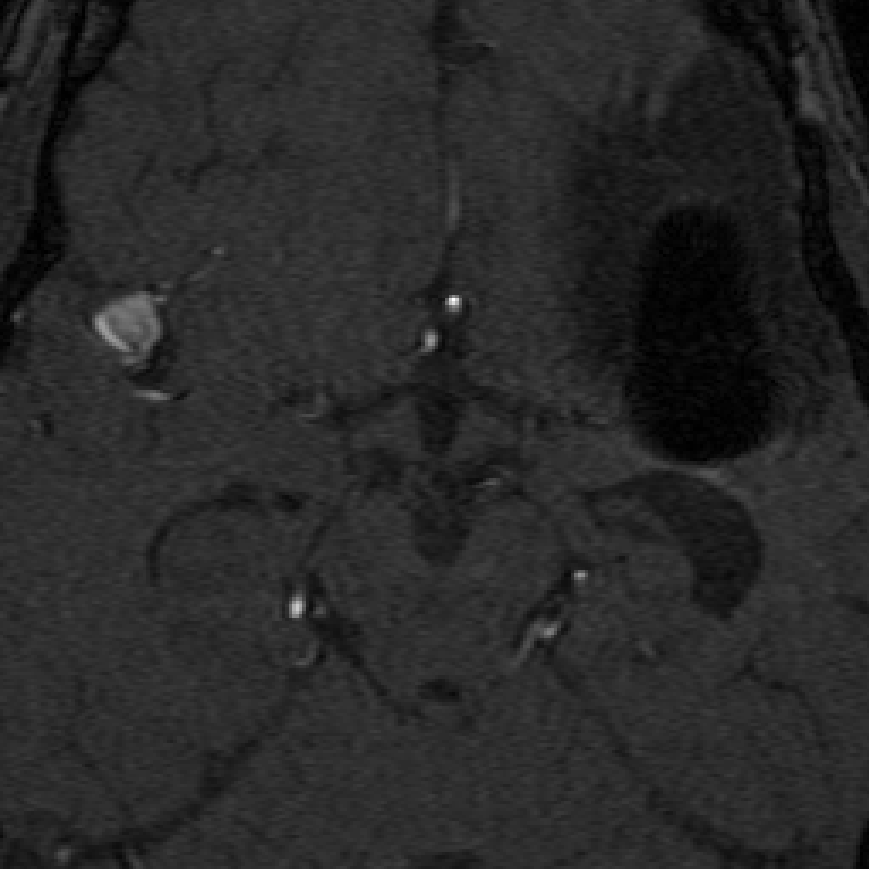
\includegraphics[width=0.5\linewidth]{figures/tof-aneu-max.png}
		
\includegraphics[width=0.5\linewidth]{figures/aneu-max.png}
	\end{subfigure}
	\begin{subfigure}{0.9\linewidth}
		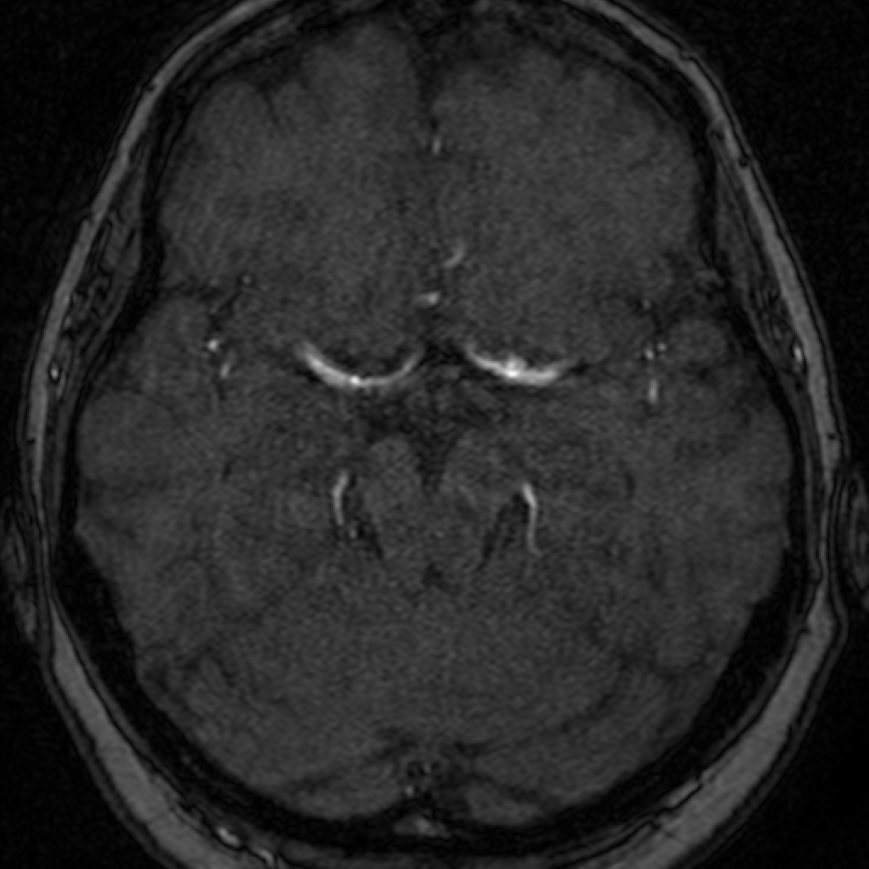
\includegraphics[width=0.5\linewidth]{figures/tof-aneu-min.png}
		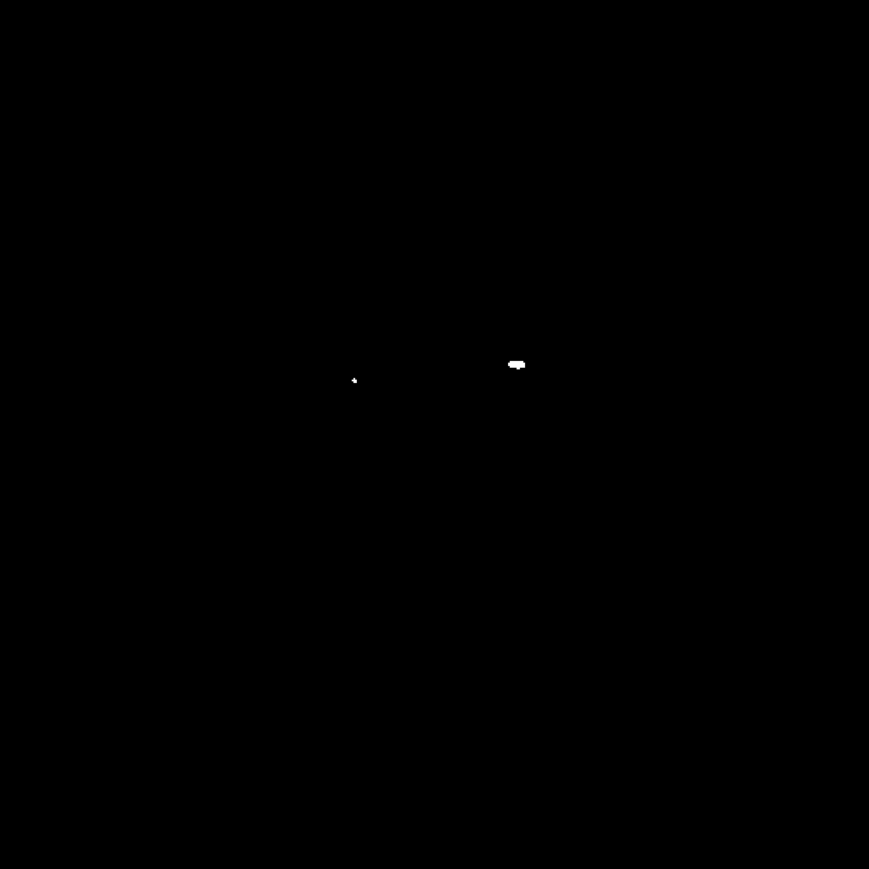
\includegraphics[width=0.5\linewidth]{figures/aneu-min.png}
	\end{subfigure}
	\caption[TOF-MRA axial slices and corresponding aneurysm label axial slices]{Axial slices of two TOF-MRA volumes (top left, bottom left) showing the largest (top right) and smallest (bottom right) aneurysm sizes.}
	\label{fig:ax-tof-aneus.png}
\end{figure}

\subsection{Dataset preprocessing}
Since the TOF-MRA volumes provided in /pre/ are already corrected for bias-field inhomogeneities this is not required. Another common preprocessing step is BET skull stripping, but this was deemed to be unnecessary in our case using this dataset. The volumes were thus resampled to a voxel to a size of $0.3 \times 0.3 \times 0.3$ mm\textsuperscript{3}, and their intensity normalized to zero-mean, unit-variance. This preprocessed data is used for training of all networks shown in the following chapters.

\subsection{Comparison to other modalities}
The imaging modalities widely used in the diagnosis of intracranial aneurysms is intra-arterial digital subtraction angiography (IADSA), computed tomography angiography (CTA), and magnetic resonance angiography (MRA). IADSA involves the use of a catheter that is advanced in the arterial system to the point of interest, and contrast material is injected while acquiring images. The contrast fills the lumen of the arteries and thus the vessel anatomy is visualized on the image. CTA involves obtaining a normal CT scan while intravenous contrast material is injected, that appears white on the CT-image due to its radio-opaqueness. The 3D reconstruction of the vascular anatomy is made digitally after analyzing serial axial slices \cite{Keedy2006}.

IADSA is widely regarded as the gold standard for intracranial aneurysm detection, due to its high spatial resolution. However, in comparison to IADSA and CTA, TOF-MRA does not require the use of intravenous contrast material, as the signal obtained during imaging depends on the magnetic properties of the area being imaged. IADSA is also costly, time-consuming and invasive. CTA also has some advantages over MRA; CTA is widely available, less susceptible to motion artifacts, and in a clinical setting it can be performed directly after subarachnoid hemorrhage is detected. Due to these reasons, it is recommended to use either CTA or TOF-MRA for pre-surgical screening, and UIA monitoring \cite{Keedy2006, Sailer2014, Wardlaw2000}. TOF-MRA is also well-suited for routine follow-up imaging as it does not need any contrast agent or radiation \cite{Lane2015}.

%\todo{Get images of each modality?}
